

The table \ref{table-spkshow-perf} shows the average $Fm$ per $SpkShow$ for the different systems.
\begin{table*}[t]
\begin{center}
\begin{tabular}{r||c|c|c}
& Percol & Qcompere & Soda \\\hline\hline
average $Fm$ & 0.361 & 0.381 & 0.351\\\hline
average $Fm$ for in dictionary speakers & 0.628 & 0.684 & 0.619\\\hline
\#$SpkShow$ out of dictionary & 200 & 209 & 204 \\\hline
\#$SpkShow$ in dictionary & 277& 268 & 273\\\hline
\#$SpkShow$ in dictionary, with $Fm=0$ & 79 & 63 & 86\\\hline
\end{tabular}
\caption{Average system performances per $SpkShow$}
\label{table-spkshow-perf}
\end{center}
\end{table*}

From the table we can notice the important number of $SpkShow$ which are not in the dictionary of the system, about 40\% for each system. As they don't have any model, they obviously cannot be identified, leading to an average global $Fm$ rather poor. More interestingly, the number of $SpkShow$ which are actually in the dictionary and which are not recognised at all, is not negligeable: their represent between 23.5\% to 31.5\% of the in-dictionary $SpkShow$, according to the systems.


Figure~\ref{fig:FMeasureDistribution} plot the distribution of all the $SpkShow$ in the system dictionaries, according their performance $Fm$, for the different systems. Foreach $Spkshow$, the average performance and the maximal performance obtained across systems are computed, and the corresponding distribution are also plotted. We can see from this figure that the average performance (from 61.9\% to 68.9\% according to the systems) presented in table\ref{table-spkshow-perf} is not at all representative of the performances obtained foreach $SpkShow$: speakers are either not recognized or well recognized. Indeed, if we compute the average performance for $SpkShow$ which have $Fm \neq 0$, the average $Fm$ grows to 87.9\% for PERCOL, 89.5\% for QCompere and 90.3\% for SODA. 

% \begin{figure}[!h]
% 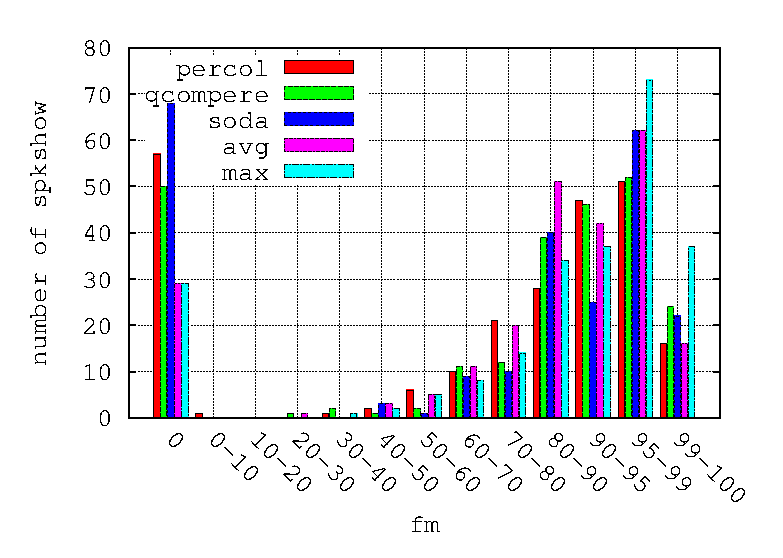
\includegraphics[scale=0.6]{figures/PQS-mono-model.eps}
% \caption{$spkShow$ performance distribution, for each system}
% \label{PQS}
% \end{figure}

To evaluate the impact of the automatic speaker diarization, we also perform the speaker analysis performance, for systems applied on reference speaker diarization. Results for systems PERCOL is shown in Figure~\ref{fig:autoVSref}.  


\begin{figure}[t]
\centering
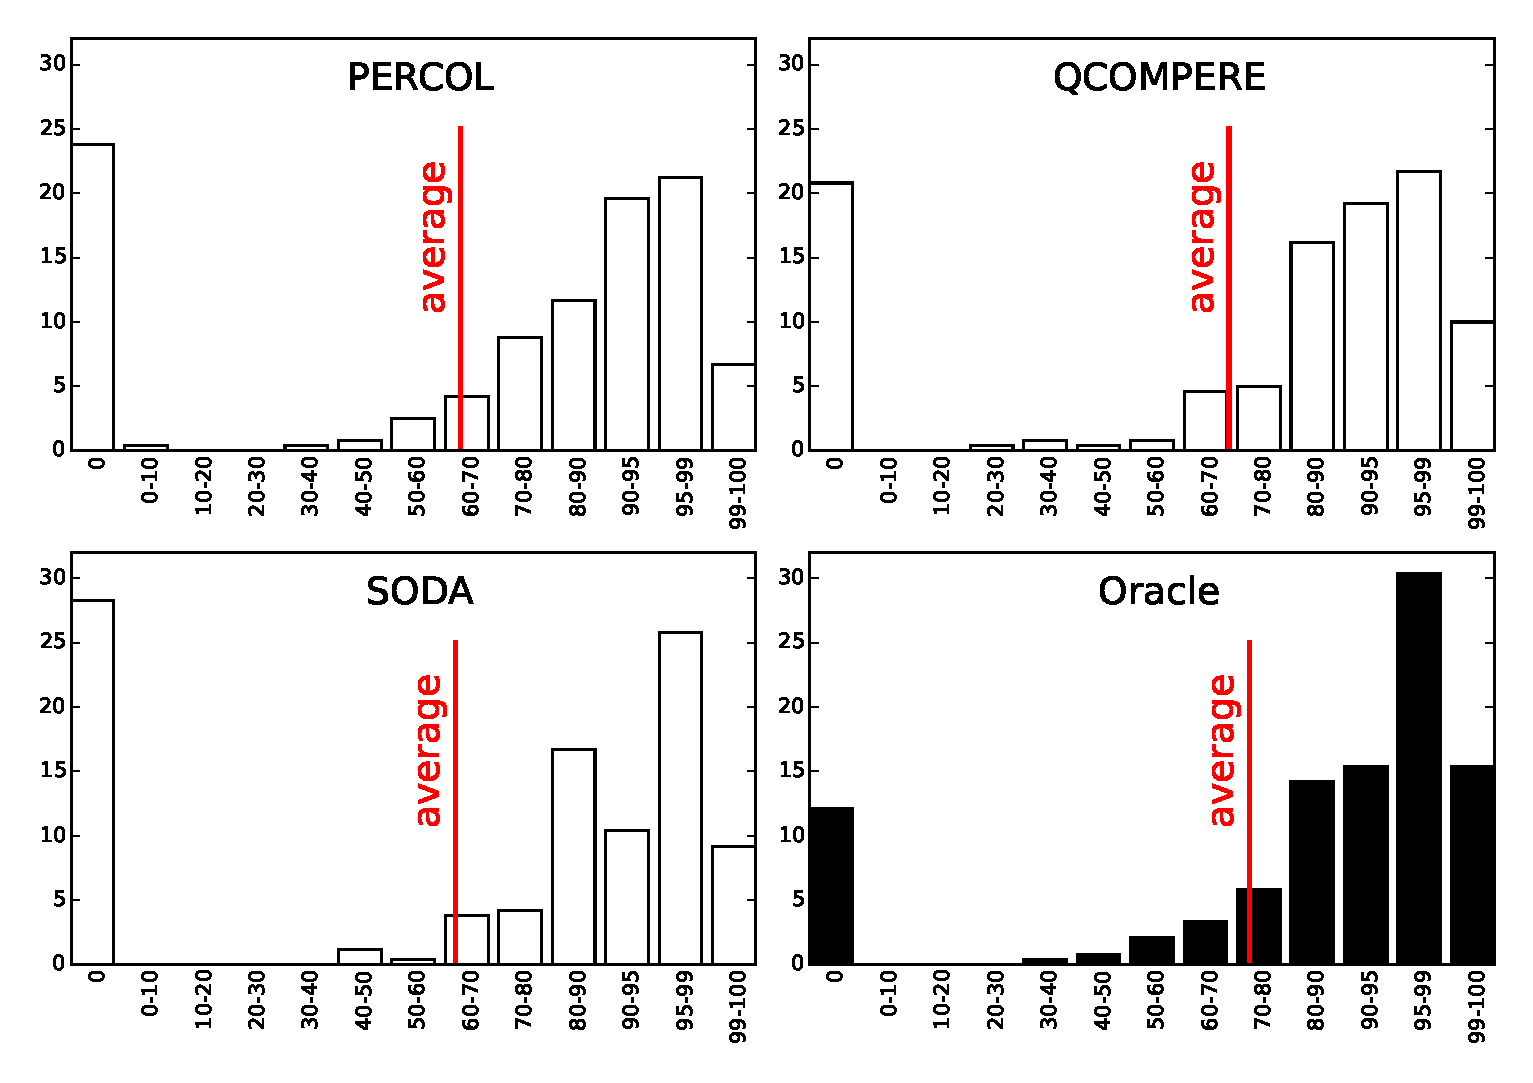
\includegraphics[width=\linewidth]{figures/bimodal.eps}
\caption{Distribution of $SpkShow$ according to system performance}
\label{fig:FMeasureDistribution}
\end{figure}


\begin{figure}[t]
\centering
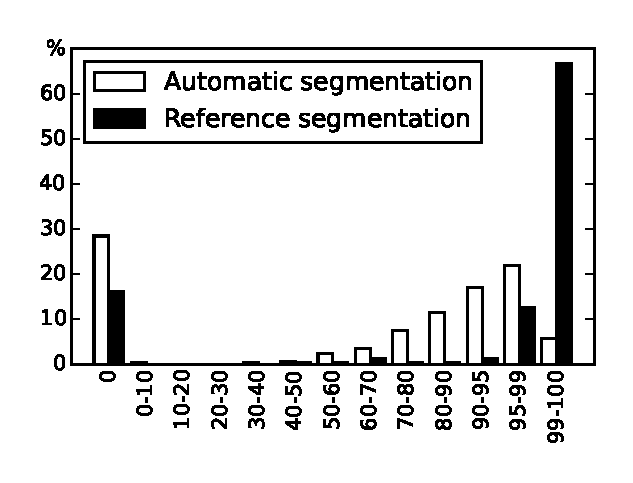
\includegraphics[width=0.7\linewidth]{figures/ref.eps}
\caption{Effect of segmentation errors}
\label{fig:autoVSref}
\end{figure}

